\documentclass[letterpaper,twocolumn,10pt]{sig-alternate-10pt}

\pdfpagewidth=8.5in
\pdfpageheight=11in

\usepackage{epsfig,xspace,url}
%\usepackage{authblk}
\usepackage{epstopdf}
\usepackage{color}
\usepackage{graphicx}
\usepackage{times}
\usepackage{multirow}
\usepackage{multicol}
\usepackage{balance}
\usepackage{listings}
\usepackage{texstuff}
\usepackage{subfigure}

\newcommand{\pubsub}{Kafka}
\newcommand{\name}{Mercury}
\newcommand{\comment}[1]{}

\title{\name{}: A Geo-Aware Mobility-Centric Messaging System}

\numberofauthors{2}
\author{
  \alignauthor Teja Kommineni\\
  \affaddr{teja.kommineni@utah.edu}
  \alignauthor Kirk Webb\\
  \affaddr{kwebb@cs.utah.edu}
  \sharedaffiliation
  \affaddr{School of Computing}\\
  \affaddr{University of Utah}\\
  \affaddr{50 S. Central Campus Drive}\\
  \affaddr{Salt Lake City, UT - 84112}
}

\def\sharedaffiliation{%
\end{tabular}
\begin{tabular}{c}}

\begin{document}

\maketitle

{\it The target call for papers is MobiSys 2017: 
\begin{verbatim}https://www.sigmobile.org/mobisys/2017/cfp.php\end{verbatim}}

\begin{abstract}
Intelligent Transportation Systems require a communication conduit for
the agents in the ecosystem. A variety of safety- and consumer-service
messages are useful, even critical for coordinating the ongoing state
of mobile endpoints.  Communicating telemetry between these endpoints,
along with data from other devices in the environment, allows them to
work together and improve safety. Moreover, it is important for
centralized services to have a global view and provide information
based on this vantage point. To this end, we have developed \name,
an end-to-end messaging system with lightweight state overhead and
publish/subscribe functionality. \name is designed to flexibly
integrate into the mobile network environment under which it is deployed.
\name's centralized Broker allows for data aggregation services and
data analysis. The Adapter tunes to the particular network
environment, allowing Client Endpoints a pathway to
communicate. Concurrent processing and event-driven design are used to
minimize latency to meet demanding low-latency messaging requirements.
\end{abstract}

\section{Introduction}

Intelligent Transportation Systems (ITS)~\cite{zhang2011data} is an emerging
area that includes many ideas and mechanisms for improving the safety,
quality of experience, and communication capabilities of
commuters. One particularly important aspect of ITS is
vehicle-to-vehicle and infrastructure-to-vehicle
communication. Vehicle area networks (VANETs)~\cite{hartenstein2008tutorial} have been
introduced to meet the challenges of mobile network actors with
rapidly changing associations arising from dynamic proximity to
infrastructure and other vehicles. Together with mobile networking a
la the 3GPP evolved packet system~\cite{4G}, robust communication
approaches involving hybrid LTE and 802.11p~\cite{802.11p} with
dynamic multi-hop clustering have been
proposed~\cite{ucar2016multihop,wolny2008modified,zhang2011novel}.
Considering safety and
other types of information exchange in an ITS, applications and events
have been identified that should be supported~\cite{camp2005vehicle,papadimitratos2009vehicular}, along
with constraints such as latency for delivery and scope
(radius). Publish-subscribe systems provide a means to efficiently
distribute messages and events between infrastructure and mobile
actors in an ITS. Such pubsub systems can support peer-to-peer and
infrastructure-sourced messages at scale~\cite{nasim2014mobile}.  While
research has been done in the areas of VANET communication and
mobility-aware publish/subscribe systems, holistic compositions of
these technologies is lacking.

Transportation safety issues are also considerable.  The total number
of vehicle sales in the United States averaged 15.43 million from 1993
up through 2015. The year 2015 saw a surge in sales, which climbed to
17.76 million vehicles and is expected to rise with the improving
economy~\cite{tradingeconomics}. Increasing vehicle populations will likely result
in increasing accident rates. A total of 32,675 people died in motor
vehicle crashes in 2014~\cite{iihs}. We argue that technology advances
should be used to mitigate increasing casualties and ensure safe
journey. A key focus in this paper is using state-of-art
5G~\cite{5gvision} networks to capture vehicle telemetry and pass
along safety events to vehicles that are relevant to their
surroundings.

The setting in which any transportation messaging system operates
requires reliable, fast paced communication. However, the latency
incurred by present solutions is not adequate for time-sensitive
interactions (e.g., for real-time inter-vehicle
notifications). Although there are architectures~\cite{ucar2016multihop} that use
the 802.11p communication paradigm for low latency, they lack good
trust mechanisms. Such ad-hoc networks are also often unstable,
requiring frequent communication path adjustments that result in
losses and overhead. 3GPP-style mobile networks provide advantages in
stability, reachability, and security.

This paper introduces \name; a integration of pubsub systems and
client endpoint mechanisms for low-latency message transport.  Part of
the holistic vision that \name{} espouses is mobility-specific
geographic areas of interest (AOI). These areas map to slices of
physical locality that are relevant to particular events.  For
example, a traffic accident and resulting congestion are relevant to
vehicles en route to the accident location, back past potential
egresses to alternate routes.  \name{} takes into account
location-specific context to calculate the relevant dynamic set of
vehicles for message transmission.

This paper makes the following contributions:
\begin{itemize}

\item A holistic end-to-end messaging system design.

The design of \name{} highlights the mechanisms by which
publish/subscribe systems and mobile endpoints can be realized in 4G
or 5G mobile network systems. Broker aggregation services communicate
through Adapters to Client Endpoints at the edge. \name's design
accommodates flexible deployment scenarios.

\item A prototype implementation and evaluation of the \name{} ITS
  messaging system.

We implemented a prototype of the \name{} components and evaluated it
on the PhantomNet~\cite{banerjee2015phantomnet} testbed.  This
prototype makes use of OpenEPC~\cite{corici2010openepc} version 5,
including its simplified emulated radio access network (RAN)
environmnet. We drive the evaluation of \name{} with our own mobility
simulator, and report on the former's functional and latency
characteristics.

\end{itemize}

The remainder of this paper is organized as follows: Section 2 covers
background, including putting \name{} into context within related
work, introducing mobile networking environment concepts, and
describing the vehicular endpoing context. Section 3 provides an
overview of the design goals and components of \name, while section
4 delves into the details of the design. Section 5 looks at how
\name{} can be positioned within different mobile networking
deployments.  Section 6 briefly discusses the \name{} prototype
implementation. We cover our vehicle simulator and provide an
evaluation of the prototype in section 7. Section 8 discusses
observations resulting from the design and implementation of \name,
and where we think it should go next.  Finally, section 9 concludes.

\section{Background}

The mobile network ecosystem is complex, and host to a number of
related efforts in providing context-specific messages between
endpoints in an Intelligent Transportation System environment. Before
we discuss the design and implementation of Mercury, we discuss it in
the context of prior work. In addition, we provide backround on the
3GPP 4G Evolved Packet System~\cite{4G}, which is an important and
widely used mobile networking ecosystem that we position Mercury
within.

%
% RELATED WORK
%
\subsection{Related Work}

There has been plenty of attention paid to effecient and reliable
delivery of messages within VANETs.  Much of this focuses on multi-hop
clustering and hybrid use of evolved packet system RAN (LTE).  The
VMaSC~\cite{ucar2016multihop}, MDMAC~\cite{wolny2008modified}, and
NHop~\cite{zhang2011novel} systems attempt to form stable mobile
802.11p clusters, using the LTE network to bridge between disconnected
clusters. These solutions largely ignore the details of the mobile
core network, glossing over questions of component placement and the
resulting effects on latency. Moreover, these systems are
complimentary to \name{} in that they can be used to reduce LTE
resource contention and improve reliable transfer of messages. Such
integration would however come at the cost of additional complexity,
failure modes, and latency due to additional network path segments.

From the publish-subscribe perspective, there is a large volume of
prior work on traditional pubsub mechanisms~\cite{hartenstein2008tutorial}
\cite{mir2014lte} \cite{kim2012performance} \cite{araniti2013lte}.
This work is complementary to ours since it focuses on the useful
aspects of pubsub, which we largely wish to reuse. There has also been
work on pubsub systems focused on mobile endpoints. The
MoPS~\cite{nasim2014mobile} publish-subscribe system scales
efficiently for large numbers of clients and deals well with changing
broker association.  \name{} could replace the \pubsub system used in
the prototype with MoPS to better target mobile endpoints. However,
MoPS does not include the area of interest concept, which would
continue to be handled by the \name{} broker. A paper by
Pongthawornkamol et al~\cite{pongthawornkamol2007analysis} looks at
pubsub in the context of ad hoc wireless networks. However, this work
only performs simulations of mechanisms, and does not consider a
larger top-down vantage point (important for coordination in a large
ITS).

Location-aware messaging, or geo-routing, in vehicular networks has
been studied fairly extensively~\cite{bilal2013position}.
Nevertheless, we find that most work has only proposed and simulated
mechanisms. Furthermore, many studies look at ad hoc networks and
fine-grained positioning of endpoints within vehicle clusters.  While
such mechanisms may be helpful for real-time collision avoidance, we
argue that they tend to be overly complex and unnecessarily constrain
the communication domain to clusters of endpoints versus a central
system with a global view. The argument against centralized systems is
frequently that mobile networks are overloaded. This may be true in
instances of particularly high device concentration (e.g. music
festivals), but we found no studies showing a general lack of
available RAN resources outside of such crowded contexts.
Furthermore, in an ITS environment, vehicle populations and
anticipated growth could be used to properly size capacity.

The related work outline above focuses on particular aspects of
messaging.  To the best of our knowledge, no messaging system targeted
at mobile endpoints simultaneously incorporates aspects we consider
crucial to a holistic messaging platform for Intelligent
Transportation Systems.  Such a system should enable a global view of
endpoints to facilitate coordinated decision-making with complete
data. It should take advantage of mobile network environment
mechanisms (e.g. eMBMS~\cite{lecompte2012evolved}) to reduce overhead and 
latency. It should
consider the placement of components within the mobile network and the
impact of this placement.  Finally, an ITS messaging system should
provide a location-aware addressing mechanism. The \name{} messaging
system is designed with all of these aspects in mind.


\subsection{Mobile Networking Ecosystem}

Mercury is primarily framed in the context of the 3GPP 4G and emerging
5G mobile networking architectures. Therefore, we provide some
background on these systems.  The vast majority of mobile carriers
utilize these Evolved Packet Systems (EPS)~\cite{mobile-stats}, making
them an especially relevant environment in which to operate a mobile
messaging system.  Note that Mercury is also amenable to other
mobility-friendly network architectures, such as
MobilityFirst~\cite{mobility-first}, but we focus the discussion in
this paper on the 3GPP EPS.  The 4G system has been in active
deployment since 2008~\cite{chen2015financial}, and has undergone a
number of revisions. Also in play in some deployment scenarios (see
section~\ref{sec:deployments}) are software defined infrastructure
concepts that are expected to be prominent components in the upcoming
5G EPS~\ref{5gvision}.

The 4G EPS includes the following key service functions relevant to
Mercury: Mobility Managment Entity (MME), Home Subscriber Service
(HSS), Serving Gateway (SGW), Packet Data Network Gateway (PDN-GW or
more commonly PGW), evolved NodeB (eNodeB), and User Equipment (UE).
We will briefly describe the role of each of these components, and
their relationships with one another and with Mercury. The Mercury
architecture diagram in figure~\ref{fig:arch} shows Mercury
components in the context of a 4G EPS.

We will briefly cover the 4G components next. \textbf{User Equipment
  (UE)} typically refers to end user devices such as mobile phones,
tablets, and 4G radio equipped laptops. The Mercury Endpoint component
runs on these. The \textbf{Mobility Management Entity (MME)} is the 4G
control plane function responsible for tracking the live (dynamic)
session state for UEs. The \textbf{Home Subscriber Service (HSS)} is
essentially a database of user (subscriber) information. The
\textbf{Serving Gateway (SGW)} is the first data tunnel anchor point
that UE sessions connect through (GTP tunnels). The \textbf{Packet
  Data Network Gateway (PGW)} act as the egress point for a large
number of UE data bearers (GTP tunnels); they fan out to multiple
SGWs.  \textbf{Evolved NodeB (eNodeB)} devices are the wireless access
points of the 4G EPS. They bridge the radio access network (RAN)
through which the mobile endpoints (UEs) directly communicate with the
evolved packet core (EPC). GTP tunnels are established for each UE
between the eNodeB it is associated with and an upstream SGW.  The
eNodeB also initiates session setup and default data bearer
establishment when UEs attach, acting as a proxy for UE to MME
control plane signalling. eNodeBs covering adjacent cells coordinate
through the MME and possibly with one another to accomplish handover
as endpoints move.

\subsection{The Vehicle Environment}

\textbf{Discuss some of the important aspects of vehicles, suchs as sensors and such, here.}

\section{Design Overview}
\label{sec:design}

Delivering messages, important and casual, to mobile users and
endpoints that are interested in them is the overarching premise of
this work. Our vision for realizing an end-to-end mobile message
delivery service design principles revolve around four central
goals:

\begin{itemize}
\item Relevant content

The service should provide mechanisms to target groups of endpoints
which have explicit or implied interest in messages. A message may be
important because an end user specifically asked for the content based
on its attributes (nearby gas prices). Alternatively, a message may be
deemed relevant for the endpoint because it is related to an emergent
event (vehicle accident ahead).

\item Robust, low overhead, low latency communication

Message intent drives content delivery requirements.  For example,
different types of emergency service messages have been identified for
VANETs, each having distinct latency
requirements~\cite{camp2005vehicle}. The service should strive to
minimize latency to provide on-time delivery with headroom for outlier
delays. Messages should be categoriezed according to their relative
importance and processed accordingly (e.g., emergency info before
consumer content).

\item Flexible deployment

Adoption of the service is bolstered by adaptability to different
mobile networking environments.  Such accomodation allows for
deployment into LTE networks with different geographic EPC service
placements and degrees of maleability.  The service should allow for
centralized metropolitan area integration (CloudRAN) and distributed
edge deployment (peer-to-peer eNodeB).

\item Reuse of effective technologies

It is our contention that an end-to-end service should not supplant
existing mechanisms useful for achieveing its composition.  Indeed, it
is counterproductive to introduce new service components that induce
unnecessary changes and capital investments. The messaging service
should strive to work alongside existing mobile network protocols and
services.  Only where existing mechanisms do not provide key
functionality or do not give adequate service levels should changes be
introduced.  Such changes should be as minimal and transparent as
possible to foster compatibility and ease of adoption. On the other
hand, considering less constrained future mobile network
architectures~\cite{5gvision,venkataramani2014mobility} is also
important.

\end{itemize}

We next describe the components of the \name messaging system, along
with how they fit into the 3GPP 4G mobile networking architecture.

%%% ARCHITECTURE FIGURE
\begin{figure*}[ht]
  \centering
  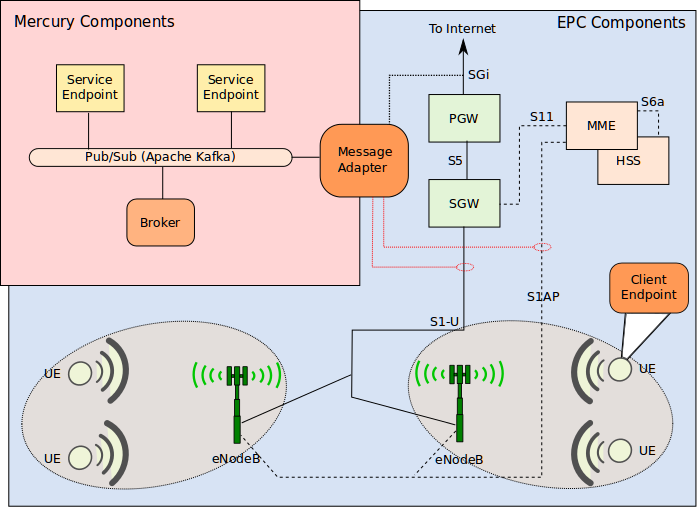
\includegraphics[width=0.8\textwidth]{figs/mercury-arch.png}
  \caption{\name architecture diagram (in 4G mobile network context)}
  \label{fig:arch}
\end{figure*}

\subsection{\name Components}

\name is comprised of four essential components: message broker,
publish/subscribe system, message adapter, and endpoints.  These
components are visible in the architecture diagram in
figure~\ref{fig:arch}. This diagram shows the \name components
in the context of a 4G mobile network (the latter will be described
after \name is covered).

\subsubsection{Message Broker}

\name's message broker is the brain center of the messaging
system. It processes all incoming messages and sends these to relevant
endpoints (via \pubsub). The broker calculates Areas of Interest (see
section~\ref{sec:aoi}) for certain message types (e.g., emergency
notifications).  Data analysis (aggregated decisions, client
statistics, etc.) occur at the broker. It does not concern itself with
how to get the messages to the target endpoint(s); that job falls to
the \name message adapter.

\subsubsection{Publish/Subscribe System}

\name needs a pubsub system that can serve a high number of events
with low latency. This is because of the environment in which it
operates.  We have many agents/endpoints at any given point that
interact with the system and for them to effectively respond to a
situation we need to dissipate the messages quickly. The mobility of
the clients creates the potential for intermitent loss of connectivity
with the pubsub system which has to be re-established. Among the options
considered, Apache Kafka had the best combination of low-latency and
message queueing for recovering lost messages.

At a high-level Kafka gives the following guarantees: Messages sent by a 
producer to a particular topic partition will be appended in the order they are
sent. A consumer instance sees records in the order they are stored in the log. 
For a topic with replication factor N, kafka will tolerate up to N-1 server 
failures without losing any records committed to the log.

\subsubsection{Message Adapter}

The \name message adapter is the conduit through which pubsub
messages flow through to endpoints. The adapter coordinates sessions
with client endpoints. It forwards client reports and other content to
and from the pubsub. It also maintains pubsub topic subscriptions for
the endpoints. The prototype implementation described in this
paper targets the 4G EPC, but it is possible to target other mobile
networking architectures with different adapters.

\subsubsection{Endpoints}

\name endpoints are the producers and consumers of most content in
the messaging system. Client Endpoints run as applications on
ITS-equipped vehicles.  They report in with telemetry, such as their
current position and speed.  Client endpoints also subscribe to
particular consumer messages identified by specified attributes.

Service Endpoints may also be centralized services that connect to the
pubsub, running at the same location as the Broker, and using the
Broker's services. Examples include emergency notification processors,
and consumer information aggregators (gas prices).

\subsection{\name Messages}

Messages are the principle and only communication mechanism in
\name. There are two high-level flavors: control and
content. Control messages include session handling (between broker and
endpoints), broker to message adapter communication, and subscription
management (endpoint to pubsub/broker).  Content messages are those
relevant to applications running on endpoints, such as emergency
alerts and consumer information (e.g. gas prices).  Periodic session
maintenance messages are sent between the mobile endpoints and the
\name Adapter to update status (location) and track liveness.

%The broker likewise sends periodic
%heartbeat messages toward all endpoints. These messages ensure clients
%and broker stay in sync. Session handling also includes establishment
%and teardown message exchange.  

Content messages use structured 
message attributes to signal category information. This allows content
producer and consumer endpoints to steer messages to one another based
on interests. Most messages (including client reports) flow through
the pubsub system to the broker. This allows the Broker to perform
data aggregation and analysis (triggers based on thresholds, for
example).

Message destination addressing in \name includes endpoint, content,
and area of interest targetting. Endpoint addresses are primarily used
for session setup and teardown. Content-specific addressing makes use
of subscription attributes to deliver messages. AOI addresses are
unique to the mobile environment. AOI bounds are computed by the
broker. These bounds form the destination address. Message adapters
check bounds to determine if their downstream area coverage is
relevant before passing along, and endpoints check their position
relative to the bounds.  In this way, \name allows messages to be
``area multicasted.''  As we discuss in
section~\ref{sec:design-details}, our prototype restricts itself to
simple bounding models (radius). Complex spatial reasoning for
improving relevancy is left for future work.

%%%%%%%%%%%%%%%%%%%%%%%%%%%%%%%%%%%%%%%%%%%%%%%%%%%%%%%%%%%%%%%%%%%%%%%%%%%%%%
%
% Old text on the pubsub that was too detailed.
%

\comment{
Apache ActiveMQ\cite{activemq} is one of the oldest player
in this space. Though, ActiveMQ messaging is reliable it's performance forms a
bottle neck to our system. RabbitMQ\cite{rabbitmq} is a widely used message 
broker with huge documentation. It is written in Erlang which is suitable for 
distributed applications, as concurrency and availability are well-supported.
However, It relies on synchronous delivery of messages that decreases the numbe
r of events being served. ZeroMQ\cite{zeromq} is another class of pub-sub 
systems that is designed for high throughput/low latency scenarios. 
Yet, most of the features will have to be implemented by ourselves combining 
various pieces of the framework. Redis is an in-memory data structure store, 
used as database, cache and message broker. Redis needs to have as much memory 
as there are messages in flight making it more attractive for short living 
messages and where we don't have a huge consumer capacity so as to not run out 
of memory.

Finally, we have crossed upon Apache Kafka. It is a pub-sub system written by 
linkedin and is under open source license of Apache. Apache Kafka addresses many
of these problems mentioned above. It is very fast and the number of 
messages/events it serves are way more than any traditional pub-sub system. 
It can handle bursts without any out of memory issues. Also, It guarantees 
event ordering. This helps us in going back in time and reading a message that
has been previously published to Kafka. We can seek old messages by remembering 
the offset. In a mobile environment this is very useful as we could see frequent
disconnections. All these attractive features made us choose Kafka as the 
pub-sub system for mercury. Below, we write briefly about different concepts of 
Kafka.

%
% Some text cut/paste from here and put into the implementation section.
%

Kafka has a beautiful concept called Consumer Groups. Consumer Groups can be 
defined as set of consumers subscribed to single topic and each consumer is 
assigned a different partition. We can have multiple consumer groups listening 
to same topic or different. This concept of forming Consumer Groups helps kafka
serve advantages of both message queue and a message-broker. Message Queues and 
message -broker systems have both strengths and a weaknesses. The strength of
queuing is that it allows us to divide the processing of data over multiple
consumer instances, which lets you scale your processing. But, queues can't be
multi-subscribed—once one process reads the data it's gone. Publish-subscribe 
allows you broadcast data to multiple processes, but has no way of scaling 
processing since every message goes to every subscriber. The consumer group 
concept in Kafka generalizes these two concepts. As with a queue the consumer 
group allows you to divide up processing over a collection of processes 
(the members of the consumer group). As with publish-subscribe,
Kafka allows you to broadcast messages to multiple consumer groups. The 
advantage of this model is that every topic has both these properties—it can 
scale processing and is also multi-subscriber—there is no need to choose one or
the other. This is something which we can take advantage of to scale Message 
Broker horizontally.


Kafka has four main APIs: The Producer API allows an application to publish a 
stream records to one or more Kafka topics. Producers publish data to the topics
of their choice. 
The Consumer API allows an application to subscribe to one
or more topics and process the stream of records produced to them. 
The Streams API allows an application to act as a stream processor, consuming an
input stream from one or more topics and producing an output stream to one or 
more output.
The Connector API allows building and running reusable producers or consumers 
that connect Kafka topics to existing applications or data systems. 
We use Producer API and Consumer API extensively in our implementation.
}

\section{Design Details}
\label{sec:design-details}

Each \name{} component runs as a self-contained application. The
Broker and Adapter(s) communicate over unmodified \pubsub. Client
Endpoints communicate with the Adapter over UDP. Client-side
applications using \name{} communicate over the local loopback with
the Client Endpoint process. Service Endpoints use \pubsub to
communicate with the Broker and talk to Clients via
Adapter(s).

\subsection{The messages and events}

The \name{} Broker we have implemented handles different types of events. 
Emergency Event, This is an event that is published by a vehicle when it senses
an emergency situation. Any message indicating such an event is immediately 
processed by the \name{} broker and sends back an area of interest (AOI)
that has to be alerted for this event.
Moving Objects Event, This event indicates that there is an object that is 
crossing a road. For such events, whenever a predicate calculated by scheduler 
evaluates to true we inform the vehicles in the AOI calculated.
There are other types of events such as Collision, Obstacle, Congestion and 
Blocked. All, these events are handled similarly but they differ in two things.
One is the predicate function and the second is the frequency at which the 
schedulers run. Our system also supports an other type of event called 
Area Of Interest. This is different from the aoi which is calculated by
\name{} broker. In this type of event the user is interested in knowing about 
the different events happening at a particular location. Whenever an event of 
type area Of interest is received by the \name{} broker. It interacts with 
different handlers and determines the bin for each event type in which the 
requested aoi falls into. Then runs a predicate on these bins and learns about 
the traffic conditions in that area which is communicated back to the user.

\begin{table*}[ht]
  \centering
  \begin{tabular}{| l | l |}
    \hline
    \textbf{Field} & \textbf{Description} \\ \hline \hline
    UUID & Unique identifier for message. \\ \hline
    Session ID & Identifies session between Client and Adapter. \\ \hline
    Message Type & Distinguishes intent (to/from Broker, PubSub, etc.) \\ \hline
    Source Address & Client ID, Service ID, Broker, or Adapter. \\ \hline
    Dest Address & Client ID, Service ID, Broker, Adapter, or AOI. \\ \hline
    Topic & Indicates topic message goes to or came from (PubSub only). \\ \hline
    KeyVal & Generic key-value \emph{pairs}. Telemetry and other data is encoded here. \\
    \hline
  \end{tabular}
  \label{tab:mesgformat}
  \caption{Message fields found inside individual \name{} messages.}
\end{table*}

Messages must fit into a single UDP packet (maximum of 64K).  Each is
self contained, with required identifiers, addresses, and message
payload.  There are two top-level types of messages in the \name{} system: 
session and pubsub.  Session messages are transmitted between
Client Endpoints and associated Adapters.  Pubsub messages can
essentially be exchanged between any \name{} components.
Table~\ref{tab:mesgformat} shows the fields present in \name{} Session
and PubSub messages. Each \name{} Address contains a destination and
source address.  The source address can be an Adapter, a specific
Client, a Service, or the Broker.  The destination address can be any
of those listed for source, and additionally may be a broadcast (all
clients, or Area of Interest geo-address).  Each message contains
key/value pairs in the payload which are interpreted by specific
applications. For example, emergency alerts published by the Broker
may be consumed by an alert display application at the Client
Endpoint.  Client Report message contain mobile telementry
information: GPS location, direction, and speed. These reports have
semantic meaning to \name, and so are tracked by the Client
Endpoint, Adapter, and Broker components.  In our prototype
implementation, the Broker has had emergency event message handling
folded into it's logic.  Therefore, the prototype Broker also
interprets safety messages sent via pubsub topics such as
``Collision'' and ``Object\_Hazard''. We envision that such message
handling would ultimately be moved to an external Service Endpoint
application.

\subsection{Areas of Interest}
\label{sec:aoi}

\name{} uses Area of Interest geo-addressing to target specific sets
of Client Endpoints.  When the Broker wishes to send a message that is
specific to a location context (e.g., a warning triggered from
multiple collision reports), it embeds the desired geo-address as the
destination, and sends this along with the message toward the
Clients. This message is picked up from the pubsub by the Adapters.
These check their coverage area and forward the message along to
Clients within the defined geo-address that they serve (or drop if
there is no overlap).  When an AOI-addressed message is received by a
Client Endpoint, it checks its current location to determine if the
message applies, and processes if so.

\subsection{\name{} broker}
  
\name{} Broker handles events in two steps: In the first step events
published are passed on to the respective handlers where we have a
filter that determines the different locations from which the feeds
are coming in for that specific event.This will give us the messages
published at different locations for an event.Each location can be
considered as a bin. We maintain for each bin the count of messages
published, the center point and the radius for that bin.  Whenever a
message comes into a bin it carries along the coordinates from which
this event has been published. We apply a simple mean with the
existing center point to determine the new center point. Thus, at
every instance we keep updating the center point and radius.In the
second step we have schedulers for each event that get triggered at
equal intervals based on the event type.  These schedulers empty the
bins of their respective event and run a predicate on them which is a
simple Boolean formula that checks for a condition.  A predicate is
usually defined over some aggregation function expressed on messages;
when the predicate evaluates to true, the \name{} broker publishes an
event to the system with the center point and the radius which we have
calculated for that bin. These are used to determine the area of
interest(AOI), AOI is the region that is determined by the \name{} broker
and constitutes all the clients that have to be alerted about a
situation.

\subsection{Pubsub service}

Within \name{} we require a publish-subscribe system for communication
between different entities.  This requirement directly arises from the
need for each vehicle to send and listen to particular types of
messages. Pubsub systems are well-suited for these activities as we
can publish and subscribe to different events. In our system
components such as Client Endpoints and the Message Broker publish and
subscribe to events.  Given this communication pattern, we developed
the set of requirments we need in a publish-subscribe mechanism and
surveyed available options.

As mentioned in section~\ref{sec:design}, we selected Apache Kafka as our pubsub
component. It is a distributed streaming platform which lets users to publish 
and subscribe to streams of records. Kafka is run as a cluster on one or more 
servers. The Kafka cluster stores streams of records in categories called topics.
Each record consists of a key, a value, and a timestamp. A topic is a category 
or feed name to which records are published. In our case it is the event type.
Topics in Kafka can be multi-subscribed; that is, a topic can have one or more 
consumers that subscribe to the data written to it. In our implementation
all the values written to a topic are listened by Message Broker. But, we could
extend this to different service end points listening on the same topic.

For each topic, the Kafka cluster maintains a partitioned log. Each partition 
is an ordered, immutable sequence of records that is continually appended to a 
structured commit log. The records in the partitions are each assigned a 
sequential id number called the offset that uniquely identifies each record 
within the partition. In our system we create a single partition for each topic.
As within a partition order is maintained we can traverse through records using
the offset of the record. Each partition is replicated across a configurable
number of servers for fault tolerance. The Kafka cluster retains all published 
records whether or not they have been consumed using a configurable retention 
period.

\subsection{Mobile network messaging adapter}

The \name{} Adapter follows a multi-threaded, event-driven execution
pattern. It is highly modular, with clear separation between client
state tracking, network-specific address mapping, and transport
functionality.  This allows new modes of core network communication to
be added alongside (or in place of) existing mechanisms.  Different
threads of execution handle pubsub, UDP communication, and scheduled
tasks (e.g., session checking); all are coordinated through the main
thread.

\name{} is designed so that any number of Adapters can connect to the
\pubsub system. Each will send client telemetry reports and pubsub
messages along. A single broker message sent via pubsub reaches all
connected Adapters, which filter as necessary. For example, an Adapter
will drop messages with Area of Interest destinations that do not
overlap with its coverage area. These coverage areas are configured by
the operator.
  
\textbf{Endpoint identification/tracking} The Adapter implements
client session tracking. When a client comes online, it goes through a
lightweight handshake with the Adapter. An INIT message is sent to the
adapter, which immediately responds with an ACKNOWLEDGE message. The
client includes a telemetry report in its INIT message so that the
Adapter and Broker have immediate knowledge of its current state. Each
client is provided with a session ID token that must be used in
subsequent messages.  The Adapter sends out periodic HEARTBEAT
messages to clients so that they can measure liveness in the absence
of other messages.

The Adapter maintains a small amount of state for each client. This
includes its unique ID, current mobile telemetry (no history), session
ID, and simple statistics (timestamp for last message received,
message count). The Adapter also maintains a mapping from the client's
ID to its mobile core network address. Changes in this address are
automatically detected and the mapping updated. The Adapter treats
periodic client reports as heartbeats, and resets corresponding
individual timers as these are received. Sessions are pruned after not
receiving a report for three times the reporting interval, or after
receiving an explicit CLOSE message from the client.

\textbf{Unicast UDP transport} In the prototype implementation, we use
UDP unicast packets for all communication between Adapter and Client
Endpoints. Ideally we would use eMBMS broadcasts for AOI and broadcast
(e.g. heartbeat) messages, and we plan to do so in future work. Each
UDP packet is a self-contained \name{} message. The contents are
encoded using Google's Protocol Buffers~\cite{buffers2011google} for
performance and space efficiency. For AOI destination addresses, the
Adapter calculates the set of clients to transmit a message to and
unicasts to each individually. For broadcasts, it transmits to all
clients with valid sessions.

\textbf{Pubsub passthrough} Messages from established clients that are
intended for the pubsub system are directly published to the indicated
topic by the Adapter. Likewise, messages received from the Broker via
pubsub are sent to specific endpoints or broadcast to all clients
handled by the Adapter (as appropriate).
    
\subsection{Client Endpoint mechanisms}

The \name{} Client Endpoint connects to the Adapter over UDP. It
establishes a session using a simple handshake; an INIT message is
sent to the adapter, which it replies to with an acknowledgement. The
client will continue trying to connect until it receives the
acknowledgement, backing off linearly with random jitter to prevent
synchronization with other clients (prevent in-cast overload). The
client will also try to reestablish its session if it does not receive
a heartbeat from the Adapter after three heartbeat intervals (tunable).
Messages are encoded using Google's Protocol Buffers.

The client gathers movement telemetry via the local sensors of the
device it is running on and sends these along periodically as report
messages to the Adapter.  As mentioned, the Adapter uses these reports
to measure the liveness of the connected clients.  Some random jitter
is added initially to the report interval to again avoid
synchronization with other clients.

The client listens over the loopback interface for connections from
local applications.  Similar to what the Adapter does for its Client
Endpoints, a Client Endpoint relays subscription requests and messages
from applications through to the pubsub/broker.  Protocol Buffers are
also used between clients and applications for encoding the messages.

%%%%%%%%%%%%%%%%%%%%%%%%%%%%%%%%%%%%%%%%%%%%%%%%%%%%%%%%%%%%%%%%%%%%%%%%%%%%%%
% 
% We may not have time/space to include any goal alignment text.
%

\comment{
\subsection{Design Goal Alignment}

The remainder of the design section of the paper is dedicated to a
deeper exploration of the design of \name{} and how it aligns with the
afforementioned goals.

\subsubsection{Delivering Relevant Content}

\begin{itemize}
\item Discuss what makes content relevant, and to whom it is relevent.
\item Metric(s) for relevancy?
\item Introduce and expand on Areas of Interest (dynamic grouping).
\item Motivate and describe publish/subscribe mechanism.
\end{itemize}

\subsubsection{Reliable Communication}

\begin{itemize}
\item Differing message requirements, based on type
\item Effects of latency, minimization through proximity to network edge
\item Delivery service levels (guaranteed, best effort)
\item Robust transit mechanisms?
\end{itemize}

\subsubsection{Deployment Scenarios}

\begin{itemize}
\item Components/service designed to integrate into different deployments
\item Minimal cost/effort: pubsub/broker centrally located with PGWs
\item Incrementally closer: MTSO or metro-area (CloudRAN) deployment
\item At the edge: Deployed as a service running on eNodeBs
\end{itemize}

\subsubsection{Integrating Trust}

\begin{itemize}
\item PKI to prevent identity forgery
\item Message integrity codes to prevent tampering
\item Sequence numbers to prevent replay attacks
\item Centralized vetting by broker to detect bad behaviors/actors
\item Encryption for privacy? We should give this some thought.
\end{itemize}

\subsubsection{Technology Reuse and Integration}

\begin{itemize}
\item Composing from a good collection of parts
\item Existing pubsub, PKI, MAC/MIC, eMBMS mechanisms, SMORE
\item Working around limitations
\item Transparent interposition
\item Open possibilities in the 5G landscape
\end{itemize}
}

\section{Deployment Scenarios}
\label{sec:deployments}

%%% DEPLOYMENT SCENARIOS DIAGRAM.
\begin{figure*}[ht]
  \centering
  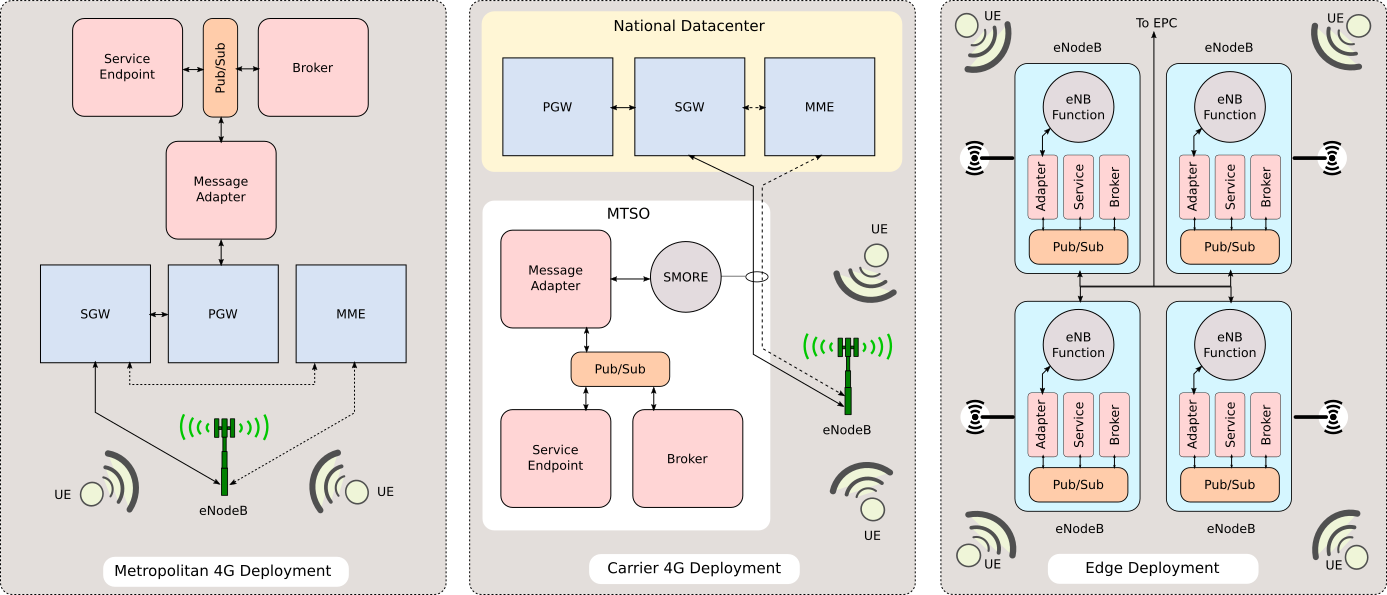
\includegraphics[width=\textwidth]{figs/deploy.png}
  \caption{\name~deployment scenarios.}
  \label{fig:deployments}
\end{figure*}

A key aspect of the \name~design is adaptability to different mobile
network deployments and architectures. Endpoints, broker, and pubsub
components are all mobile-environment agnostic. Mobile endpoint
identity is specific to the \name~messaging system. One of the message
adapter's primary functions is to separate the concerns of the
messaging system with the routing of messages inside the mobile
network.  \name~requires a low-latency vantage point near the mobile
network edge. Message adapters, pubsub, and broker all need to reside
at this vantage point.  Such proximity allows for message delivery to
meet timing requirements.  Distance to endpoints incurs a tradeoff between
convenience of deployment and ability to meet timing needs. We show
deployment versus distance/latency requirements in
table~\ref{tab:lat-req}.

{\bf ADD REFERENCES TO TABLE}

\begin{table}[h]
  \centering
  \begin{tabular}{| l | l | l |}
    \hline
    \textbf{Latency Tolerance} & \textbf{Examples} & \textbf{Ref} \\ \hline \hline
    High ($> 1$ second) & Consumer info, Congestion & \cite{camp2005vehicle,papadimitratos2009vehicular} \\ \hline
    Medium ($< 50$ msec) & Lane change assistance & \cite{FIXME} \\ \hline
    Low ($< 10$ msec) & Vehicle control loop & \cite{hansson2002integrating} \\ \hline
    \hline
  \end{tabular}
  \label{tab:lat-req}
  \caption{Latenct tolerances for different types of vehicular environment messages.}
\end{table}

The message adapter can utilize different techniques to interface with
a mobile network deployment. In the simplest case, it can interact
with endpoints via routed network addresses (e.g. IPv4 or
IPv6). Alternatively, it may transparently interpose on encapsulated
communication channels to inject/extract messages (e.g. GTP
bearers). Another option is for the message adapter to operate in
concert with the wireless access point right at the edge. It could do
this by transparently interposing on the access point's data plane
uplink, or via an integrated side channel added into the access point
software.  We next present three plausible deployment scenarios, each
of which is shown in figure~\ref{fig:deployments}.

\subsection{Metropolitan area 4G deployment}
\label{sec:metro-deploy}

Consider a city investing in Intelligent Transportation System
infrastructure. Resources include a data center within the city and
wireless coverage via eNodeBs (particularly along major vehicle
corridors). The 4G EPC components reside in the local data center,
including the PGW.  Given a maximum cabling distance from the data
center to any eNodeB of around 100~kilometers, one way speed of light
latency is bounded to less than 5~milliseconds.  LTE one-way wireless
first-hop target latency is 5~ms, but may be more like
10~ms~\cite{laner2012comparison} due to UE and eNodeB processing overhead.
Further switch/router hops within the data center should not
appreciably add to the latency. Egress through SGW/PGW can add another
5~ms of one-way delay.  Total mobile network
infrastructure RTT is thus bounded to 40~ms. This leaves 10~ms for
\name~components to process messages for low-latency
vehicle-to-vehicle coordination (within 50 ms).

In this deployment, the \name~message adapter, pubsub, and broker
all reside alongside the PGW in the local metro data center. The
message adapter and mobile endpoints communicate using native network
addresses (i.e. IPv4 or IPv6).  \name~components communicate via the
data center pubsub deployment. The endpoints can obtain the address
of their associated message adapter using DNS, DHCP options, or
multicast query.

\subsection{Existing mobile carrier 4G network deployment}

In an existing 4G mobile carrier network, there may not be a
centralized upstream network egress location in a particular metro
area of interest. Further, PGW nodes are typically deployed at a
handful of national data centers.  Total one-way latency to egress
through a PGW in such deployments is often over
50~ms~\cite[Chapter~7]{grigorik2013high}. Installing \name~at these national
data centers would impair its ability to meet SLAs for some classes of
low-latency messages (see table~\ref{tab:lat-req}). Many mobile
carriers, however, concentrate regional connectivity at a Mobile
Telephone Switching Office (MTSO).  Typical one-way latency from
eNodeB to MTSO is 10~ms~\cite{cho2014smore}. With LTE RAN latency
added, the one way latency between MTSO and UE is about 20~ms.

Deployed into a MTSO, \name~message adapters can interpose on GTP
data bearers for UEs in the same way that SMORE~\cite{cho2014smore}
does. Alternatively, lower-capacity (thus cheaper) combined SGW/PGW
functions may be deployed into the MTSO. This would allow the provider
to setup dedicated bearers for services such as \name~in a MTSO
location.  Using these options, \name~can operate with slightly
higher RTT compared to metropolitan data center deployments.  However,
the additional latency may not meet the latency requirements for some
UE-to-UE (vehicle-to-vehicle) applications.

\subsection{Mobile edge 4G/5G deployments}

\name~can be altered to run at the network edge, on the mobile
wireless access points.  If a deployment includes the ability for
running services on the eNodeB (or equivalent) access points, then
\name~can operate using peer-to-peer semantics.  All components of
\name~would run on each eNodeB, and some service endpoints as
well. The pubsub is extended to form a connectivity mesh between
adjacent eNodeBs. \name's scope at each eNodeB is smaller, and so
the amount of processing is reduced. When a message destination is an
area of interest, the local \name~broker determines whether parts of
this area lie outside of its coverage.  If so, it sends such messages
along (via pubsub mesh) to neighboring eNodeBs. These handle their
portion of the endpoints in the AOI.  Arbitrary consumer content
messages are also sent along to potential subscribers via the pubsub
mesh.  This deployment scenario allows for very low-latency messaging
between nodes connected via the same eNodeB (potentially under 20~ms
RTT considering RAN latency). Inter-eNodeB communication latency
depends on the communication path between eNodeBs.  This could be only
a handful of milliseconds if there are metro-area-local paths.

A second realization of this deployment scenario is via a 5G CloudRAN
environment~\cite{checko2015cloud}. Here eNodeBs are split into remote radio
heads (RRH) connected to base band units (BBUs).  The latter are
located in nearby compute aggregation locations; RRH and BBU functions
can only be about 25~km apart in order to maintain the closed control
loop between them. BBU functionality in a compute location serves
multiple RRH units. \name~components would be deployed into the
compute locations in this case.  Multiple such compute locations may
serve an area. \name~could be deployed to each with a peer-to-peer
pubsub mesh setup between them.  Similar very low latency messaging is
possible in this scenario with a \name~message adapter working with
the BBUs at its location.  An additional advantage is that the very
low latency messaging extends to the (larger) area covered by all
associated RRH units.

\section{Implementation}

We next briefly cover some of the essential implementation details of
the Mercury prototype. Section~\ref{sec:design-details} discusses our
selection of Kafka for the pubsub component. Google's Protocol Buffers
were used for efficient on-the-wire binary encoding of messages. Such
encoding is used on all non-pubsub communication paths. The Mercury
prototype was written in python in about 2,200 lines of code. We chose
Python because it was easy to rapidly produce a working system in this
high-level langauge, and because it has good support for parallel
processing. Integrations exist for Python for the other technologies
used. Concurrent threads are employed to capture and buffer incoming
messages from both the pubsub and UDP point-to-point channels. An
internal scheduler was implemented to perform periodic tasks, and
supports randomized offsets.

The prototype implementation targets the centralized PGW deployement
scenario where the core Mercury components (Adapter, Broker, and
pubsub) are positioned immediately on the other side of a standard
3GPP data bearer egress point. This deployement scenario affords low
latency overhead when EPC core components are located in a datacenter
near the network edge.  We covered this deployement scenario in
section~\ref{sec:metro-deploy}.  Note that we did not take advantage
of any specific aspects of the mobile environment in our prototype,
which is left as future work.

\section{Evaluation}

\begin{itemize}
\item Discuss evaluation approach.
  \begin{itemize}
  \item Do evaluation in PhantomNet using OpenEPC with emulated RAN.
  \item Use vehicle mobility model, SUMO, to drive realistic mobility scenarios.
  \item Use SUMO output (position, primarily), to trigger handover.
  \end{itemize}
\item Types of evaluations to perform.
  \begin{itemize}
  \item Functional: Endpoints connect and are tracked properly (handover).
  \item Functional: Areas of Interest are interpreted properly.
  \item Scaling: Run simulated/emulated scenarios with dozens of endpoints.
  \item Scaling: Increase message/sec load and observe system response times.
  \item Trust: Try to forge and alter messages (MITM)
  \item Trust: Try to manipulate system state (``i.e., game the system'').
  \end{itemize}
\end{itemize}

\section{Discussion}

The design of \name, the possible deployment scenarios it can
accommodate and the evaluation of prototype implementation of \name{} 
clearly suggest that \name{} is a fit for both present and future
Intelligent Transportation Systems. Yet, there are few areas where we
can further improve to make \name{} more appealing.

At present, \name{} uses AOI as a main primitive in delivering
messages to the clients. \name{} Broker determines the AOI and this is
processed by the Message Adapter to deliver messages to respective Clients.
The AOI that we are implementing or envisioned in this paper is based
on the circle centered at a point with a given radius. Clearly, when
we are using the circular region as metrics there could be vehicles
which are not affected by the event yet receive the alert message from
\name{} because they fall inside this region. This is where we think
AOI calculation should also add another dimension to its measurement,
namely direction. This comes from the basic concept that an event
happening on one side of the road may or may not affect the vehicles
moving on the other side of the road. Looking at the directions we can
also detect collisions between vehicles using the reports they send to
the system.  Hence, this is an interesting future work area.

Presently, the Message Adapter doesn't implement any significant
security measures when dealing with the messages that are moving in
and out of the system. We only check if the sender of the message has
a session with \name{} and then forward it to the \name{} Broker. The
verification that is done here can be further supplemented by other
methods such as self-certifying endpoint IDs and signed messages (to
prevent spoofing), and data analysis at the Broker looking for
anomalies (to prevent gaming).  Without such protections, miscreants
could exploit and/or spoof messages without sensing an event or in any
other anticipated way that could generate profits to them or cause
harm to others.

The Message Broker receives all sensed events from the Message Adapter
and performs computation on them to determine AOI. Here, we can see
that Message Broker depends on the incoming messages to figure out
whether an incident/event is happening. It doesn't have any other way
to know about an event except for the incoming messages. But, if we
have a close look at \name{} we also have another source of
information; the reports that are periodically sent by vehicles.  We
can make the Message Broker intelligent enough to look at these
reports and detect an event. It could further decrease the latency in
the system and we could make more informed decisions a step before a
threshold of vehicles get to sense this event and report it to the
system. For example, all vehicles which are in a region experiencing
congestion move at a slow speed. Looking at the reports from vehicles,
we could detect the slowing down of vehicles in any region and send a
congestion alert to relevant vehicles (via AOI).

Section~\ref{sec:deployments} mentions a handful of different
deployment scenarios. We would like to extend \name{} into these
different scenarios and measure its performance. In particular,
we would like to make use of eMBMS for broadcasting AOI and
heartbeat messages to Clients.  We would also like to explore
the edge deployment scenario. This scenario has the greatest
potential for minimizing latency, and also has interesting fault
tolerance properties and challenges. Keeping a mesh of agents
running at each eNodeB bypasses issues in the core network, but
means manging message routes and maintaining healthy paths.

Finally, there are a number of things we can do to improve the
performance of \name. We could increase the performance by increasing
parallelism in the system such as scaling Message Adapter and Message
Broker. We could also take advantage of the consumer groups concept in
the Apache Kafka that help us in instantiating multiple consumers on a
single topic. This way all the messages that come to a single topic
can also be processed by multiple consumer instances giving us high
throughput. We can also take advantage of the retention period in the
Kafka to go back in time and receive any alert if missed. This could
probably be an interesting option to look at because vehicles may tend
to lose connection to intermittently and when they establish
connection again with the system they might be interested in listening
those events that it missed.

\comment{
\begin{itemize}
\item Lessons/insights extracted from design/implementation/evaluation.
\item Future work.
\item Limitations of approach.
\end{itemize}
}

%\subsection{Related Work}

There has been plenty of attention paid to effecient and reliable
delivery of messages within VANETs.  Much of this focuses on multi-hop
clustering and hybrid use of evolved packet system RAN (LTE).  The
VMaSC~\cite{ucar2016multihop}, MDMAC~\cite{wolny2008modified}, and
NHop~\cite{zhang2011novel} systems attempt to form stable mobile
802.11p clusters, using the LTE network to bridge between disconnected
clusters. These solutions largely ignore the details of the mobile
core network, glossing over questions of component placement and the
resulting effects on latency. Moreover, these systems are
complimentary to \name{} in that they can be used to reduce LTE
resource contention and improve reliable transfer of messages. Such
integration would however come at the cost of additional complexity,
failure modes, and latency due to additional network path segments.

From the publish-subscribe perspective, there is a large volume of
prior work on traditional pubsub mechanisms~\cite{hartenstein2008tutorial}
\cite{mir2014lte} \cite{kim2012performance} \cite{araniti2013lte}.
This work is complementary to ours since it focuses on the useful
aspects of pubsub, which we largely wish to reuse. There has also been
work on pubsub systems focused on mobile endpoints. The
MoPS~\cite{nasim2014mobile} publish-subscribe system scales
efficiently for large numbers of clients and deals well with changing
broker association.  \name{} could replace the \pubsub system used in
the prototype with MoPS to better target mobile endpoints. However,
MoPS does not include the area of interest concept, which would
continue to be handled by the \name{} broker. A paper by
Pongthawornkamol et al~\cite{pongthawornkamol2007analysis} looks at
pubsub in the context of ad hoc wireless networks. However, this work
only performs simulations of mechanisms, and does not consider a
larger top-down vantage point (important for coordination in a large
ITS).

Location-aware messaging, or geo-routing, in vehicular networks has
been studied fairly extensively~\cite{bilal2013position}.
Nevertheless, we find that most work has only proposed and simulated
mechanisms. Furthermore, many studies look at ad hoc networks and
fine-grained positioning of endpoints within vehicle clusters.  While
such mechanisms may be helpful for real-time collision avoidance, we
argue that they tend to be overly complex and unnecessarily constrain
the communication domain to clusters of endpoints versus a central
system with a global view. The argument against centralized systems is
frequently that mobile networks are overloaded. This may be true in
instances of particularly high device concentration (e.g. music
festivals), but we found no studies showing a general lack of
available RAN resources outside of such crowded contexts.
Furthermore, in an ITS environment, vehicle populations and
anticipated growth could be used to properly size capacity.

The related work outline above focuses on particular aspects of
messaging.  To the best of our knowledge, no messaging system targeted
at mobile endpoints simultaneously incorporates aspects we consider
crucial to a holistic messaging platform for Intelligent
Transportation Systems.  Such a system should enable a global view of
endpoints to facilitate coordinated decision-making with complete
data. It should take advantage of mobile network environment
mechanisms (e.g. eMBMS~\cite{lecompte2012evolved}) to reduce overhead and 
latency. It should
consider the placement of components within the mobile network and the
impact of this placement.  Finally, an ITS messaging system should
provide a location-aware addressing mechanism. The \name{} messaging
system is designed with all of these aspects in mind.

\section{Conclusion}

We have presented \name, an end-to end mobility centric messaging
system that improves safety within the vehicular environment. We have
looked at the architecture and different components of \name. We
have discussed the different deployment scenarios and how \name can
fit in each of them. We also analyzed the need of a pubsub system in
this environment and our choice to use Kafka for the
implementation. We evaluated our prototype \name implementation in a
4G deployment context. A vehicle simulator was written to test
functional correctness, and a synthetic echo application was used to
evaluate rount trip time latency performance. We conclude that the
prototype is functionally accurate, but requires additional
parallelism and tuning to meet latency requirements for realistic
workloads. We have also considered how adding a direction based metric
to this system would make it more precise and how we can incorporate
more trust into \name so that it is not misused.


{
  %\footnotesize 
  \small 
  \bibliographystyle{acm}
  \bibliography{biblio}
}
\end{document}
